\chapter{Network Management} \label{chap:nm} %% chapter 3

As networks grow larger and more complex, systems must be put in place that allow for closely monitoring the resources that make up the network, while also allowing for a certain freedom for the possible constant change of the 
network. As such, typical vendor solutions don't really fit into this ever changing landscape, since they present very solid and vertically integrated solutions. The SDN paradigm, however, is able to solve this issue, since it 
enables for the centralized control of the underlying networks, which provides for visibility and even control over the network, simplifying network diagnosis or troubleshooting. 
\par Although SDN is a promising paradigm in terms of networking management, it also introduces some points of failure that are non existing, or not as impactful in current networking deployments. This is related, for example,
to the centralization of the controller, which makes it susceptible to Denial-of-Service attacks or even the possibility of some malicious attacker that could possibly exploit the privileged view that the SDN controller has.
\par This chapter focuses on the management of networks, where we explore what is most necessary to obtain a comprehensive understanding of the network; formalize the statistics that can be reported via OpenFlow; see some 
research that has been done in the management of SDN applications, including what existing controllers provide us; and finally explore the way that DDoS detection and mitigation is usually implemented.

\par The topic of network management is very extensive, due to the several components that make up today's networks, and the vast amount of information that they provide. It can be summed up as the operation and maintenance 
of network infrastructure so that the service it provides is not only "healthy", but also is operated at a level that keeps costs down for service providers. While obviously important for all network operators, these are 
some very important concerns that should be taken care in cloud service data center networks. The modern cloud computing centers are subject to several different characteristics than more traditional infrastructures, due to the 
increasingly predominance of virtualisation of server and networks or the pretty specific topology types that can be present in these deployments,  as can be seen in figure 4.1. Other possible topologies include de Bruijn server only
networks, or BCube switch heavy networks \cite{ popa_cost_2010 }.

\begin{figure} [h]
    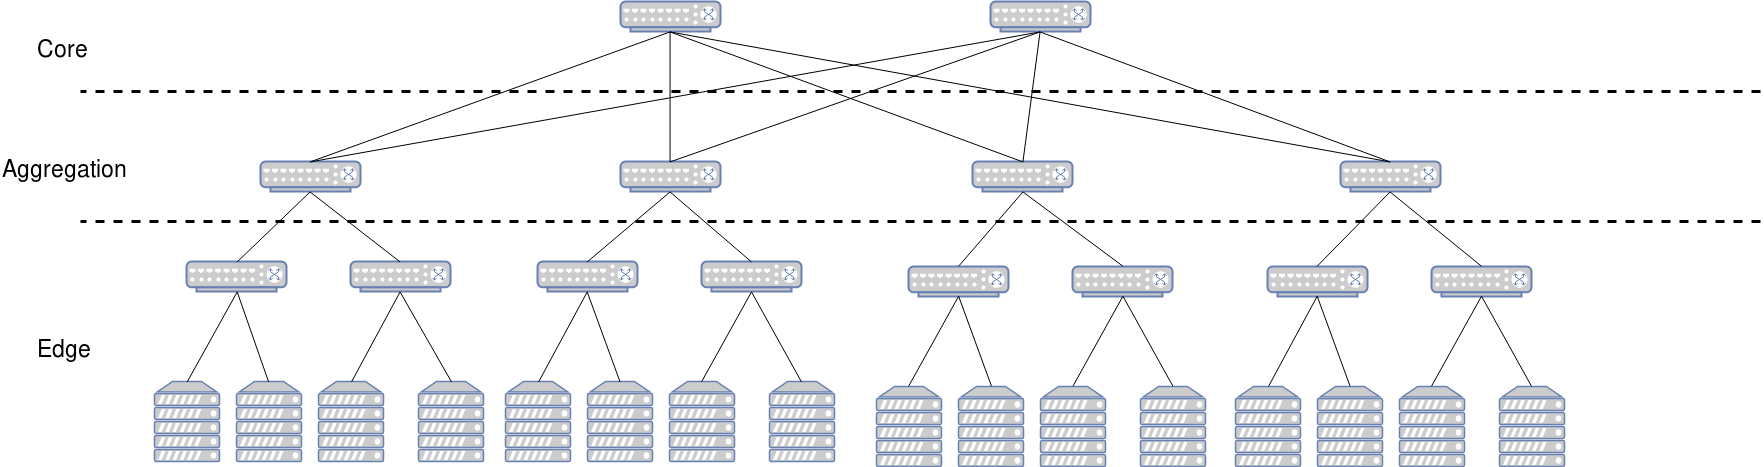
\includegraphics[width=1\textwidth]{nm/fattree}
\caption{Visual representation of the fat tree topology commonly used in data centers}
\end{figure}


\section {OpenFlow Statistics}




